\chapter{Background \& Ojectives}

\section{Background}
Real-time strategy (RTS) games have a huge market on desktop environments, but have yet to make the break through into the mobile gaming market. This is mostly attributed to the complex control mechanisms that need to be executed precisely. A mobile devices form factor restricts the number of controls that can be presented to the user at any given time as well as the precision in which these commands can be issued.

RTS games are generally designed around large, expansive maps that cover a large range of environments and landscapes. The game map shapes how the game will be played, how involved the player feels and ultimately the engagement of players. These maps can take years to develop and result in one of the largest costs within the development process. So when coming up with an environment why not take advantage of a ready made one? That of planet Earth.

Building a game where the game play takes place on a map of Earth has a number of benefits. First is the scale of a map covering 510 million square kilometres of varying terrain and features. This scale also contains a huge level of detail that could not be achieved by a team of designers. Along side this there is the feeling of familiarity, unlike when starting a new game and having to teach the player about the environment, the user will already have a well formed model in their own head. Along with highly detailed knowledge about certain areas especially those within close proximity of their current location.

Mobile devices have a whole host of unique features and sensors that set it apart from other gaming platforms. One feature that has been widely adopted in a huge range of different applications is location. A users location can be easily determined with a number of different components present on most modern smart phones, these are a GPS chip and the mobile GSM network. Although location has been used extensively in applications it has yet to be utilized effectively as a key metric within a game. This extra information about the user would enable a game set around the physical world to be able to be integrated with the user. Instead of placing new users randomly on a unfamiliar map they can be placed in their real location. Thus giving them a chance to use their own knowledge of their surroundings to help them within the game environment.


\section{Market}

A worldwide RTS game that combines a map of the world and data gathered about the user combine to create a unique gaming experience and could add an entirely new dimension to the genre. This can also reduce the learning curve and thus shorten the time between installation and engagement. With the sheer number of applications available on a mobile platform combined with the ease and minimal to no cost of installing new applications, this is important to reduce the chance of the user simply finding an alternative.

\subsection{Choosing a platform}
The current mobile platform oligopoly results in their only being two viable platforms, Apple's iOS and Google's Android OS. The Android operating system, as of February 2013, had over 51\% market share in the US\cite{smartphone_market}. Closely followed by the original and most established app ecosystem of Apple iOS. Even though there are other platforms, such as Windows phone and Blackberry, none of these have the market share allow them to be a primary platform of choice. Therefore choosing between the two platforms can be an important decision for mobile developers, both platforms offer their own unique advantages and disadvantages. Android on the one hand has the lead on market share offering a larger audience, although this will not directly affect engagement or return.

This years Developer Economics report\cite{de} looks at all aspects of the mobile app market and is an invaluable insight into both the market and consumer trends. As well as evaluating the current market it also gets feedback from developers as to their experiences with different platforms as well as their success.

\begin{figure}[H]
  \centering
   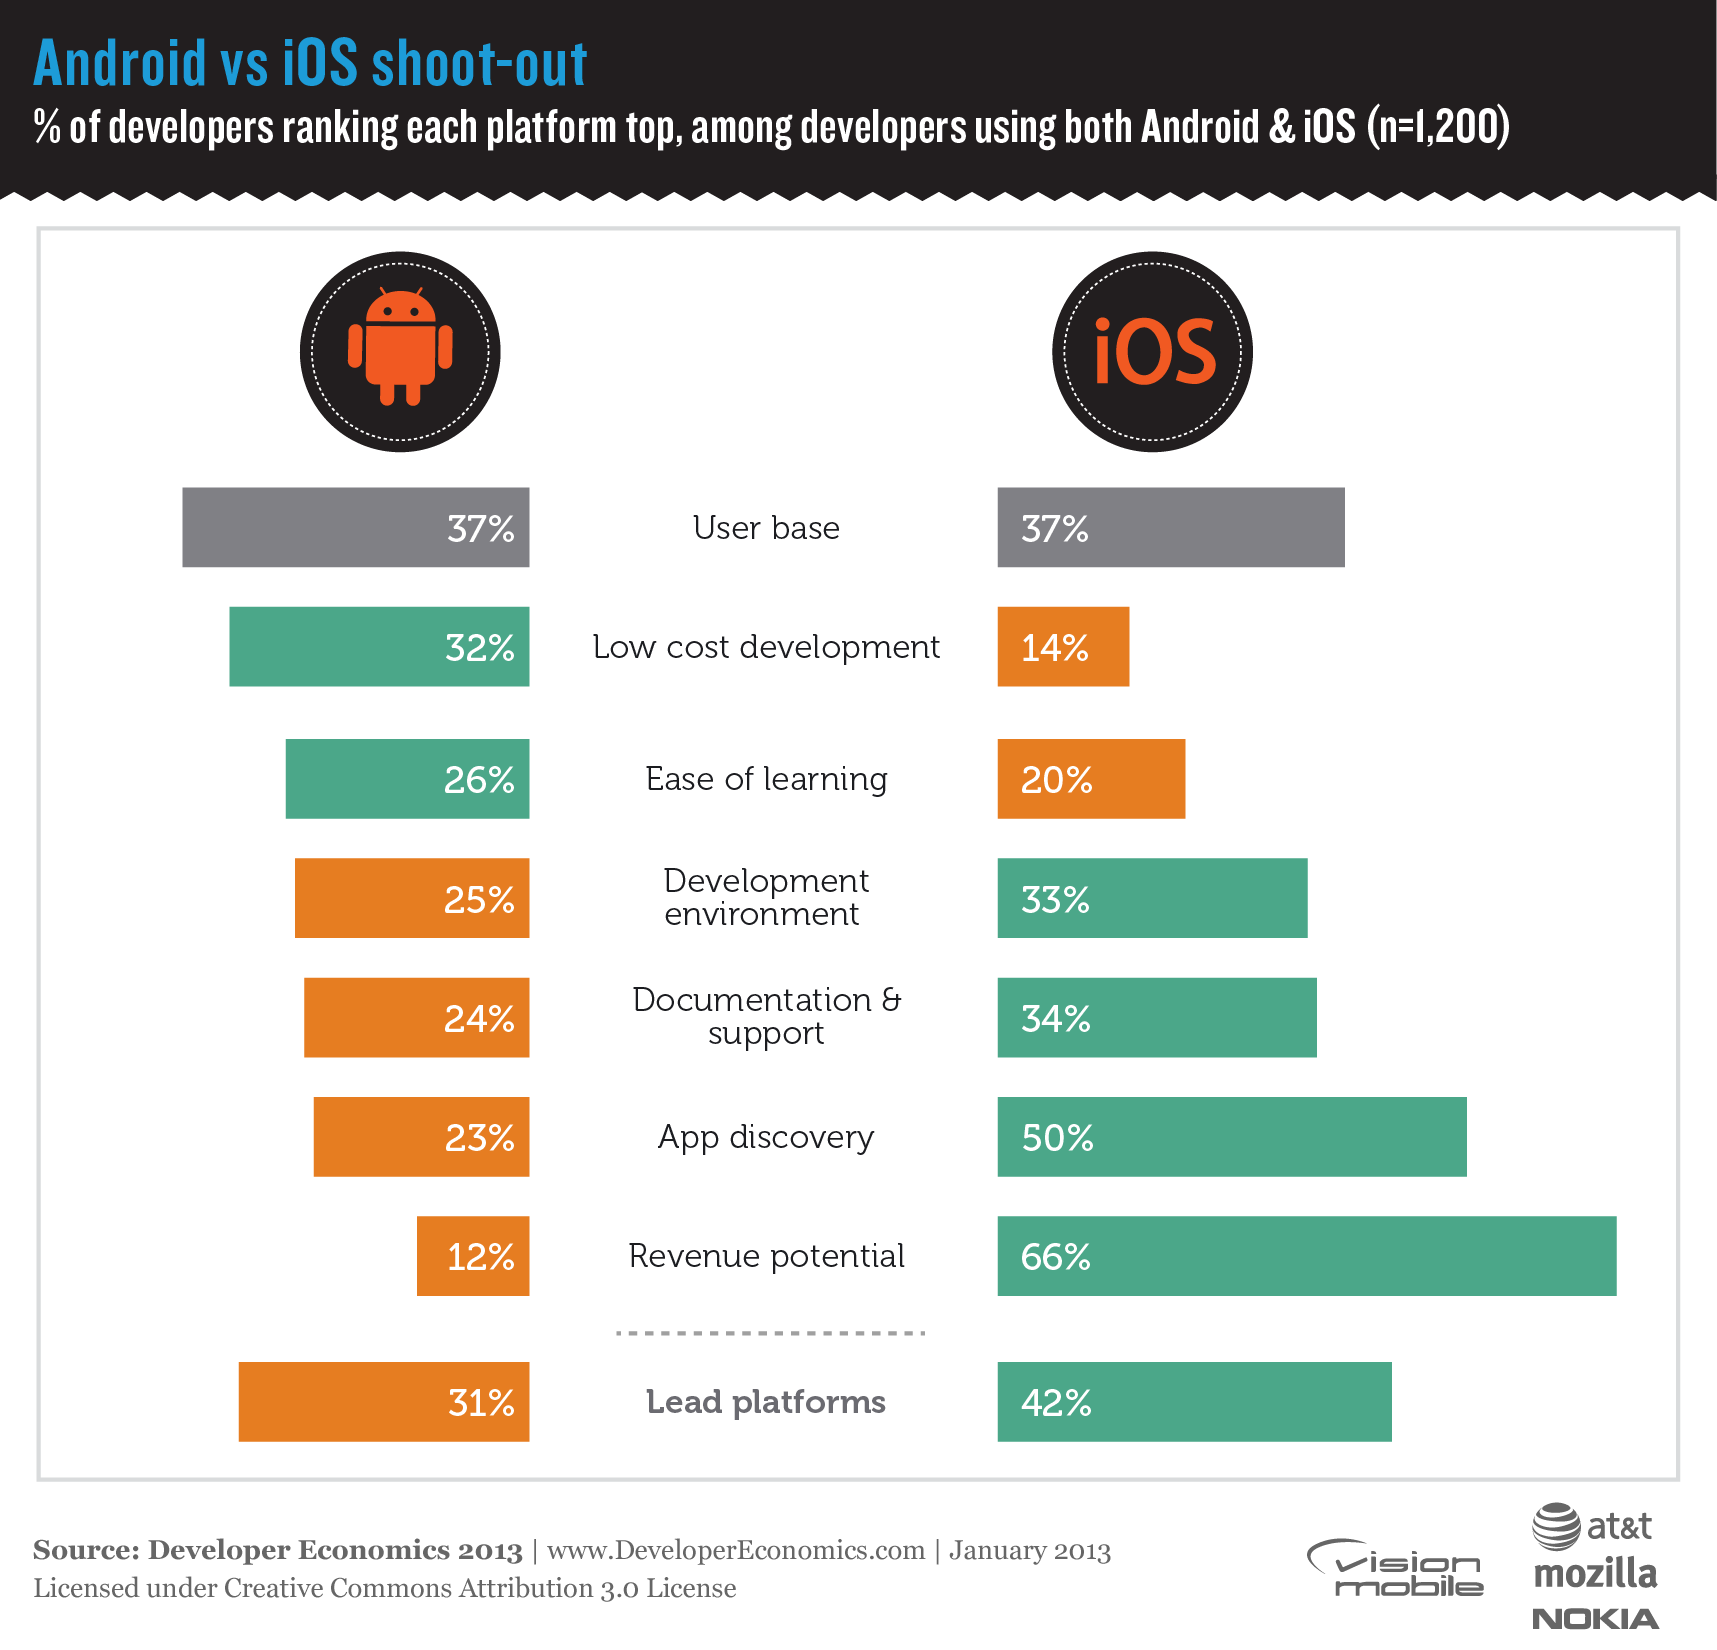
\includegraphics[width=0.8\textwidth]{Images/android_ios.png}
  \caption{Developer Economics report\cite{de} shows iOS\\as the leading platform among developers}
  \label{fig:de}
\end{figure}

As shown in Figure \ref{fig:de} iOS does indeed have a number of advantages over Android. Most importantly is the drastically increased chance of discovery as well as the expected return from applications on the iOS platform. For this project however less emphasis was placed on the success of the finished application and more on the process of creating it. Therefore the metrics of development cost and learning curve were considered to be more important. Aside from the Developer Economics findings there were a number of other more fundamental reasons as to why Android was the preferable platform. There was a certain amount of background knowledge and previous experience both with using and developing for the platform. The development environment had already been investigated and a small application developed prompting confidence in the ability to create and deploy something. Also a reasonable selection of Android devices were available for developing and testing purposes, which was favourable to using emulators and a single test device which would have been available for iOS.

The final consideration, which will be explored further in the following subsection, is that of not just overall market share but the scale of competition. IOS tends to attract the gaming market and as a result has a large selection of highly polished, top quality gaming titles. Whereas the Android market has a considerably smaller selection of games and these tend to be more basic and less graphically pleasing. Although this is changing as game developers migrate to Android it does give an advantage to new developers that might not be able to compete with the quality of iOS.


\subsection{Android RTS Games}
There is currently only a small handful of RTS games available for Android and of these most are unsatisfactory attempts. That being said there are a few well executed examples with the best examples coming from Noble Master Games (http://www.noblemaster.com/) who focus entirely on making these types of games for both desktop and mobile. The Stormfront series (http://www.operationstormfront.com) consisting of Tropical Stormfront and Desert Stormfront are the closest Android offerings to a full RTS gaming experience. Originally released for Android both were later ported to PC, MAC and Linux then subsequently iOS, this was made possible due to the game being built with OpenGL. These games offered the best chance to evaluate what had been done before and see what is expected and what would work well for MapWars. By examining different aspects from game play to control options it is a good opportunity to pick up ideas for the UI and user interaction.

\begin{figure}
  \centering
   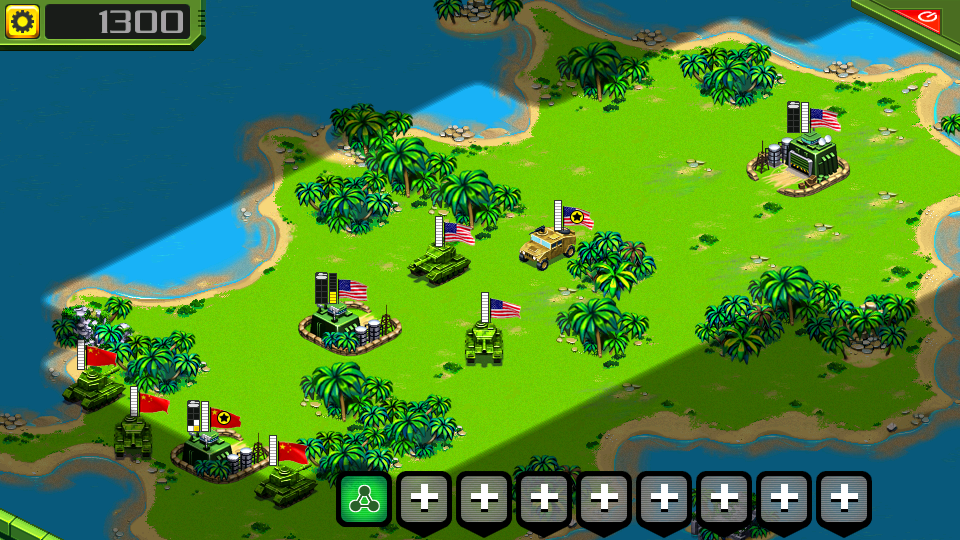
\includegraphics[width=0.8\textwidth]{Images/tropical_storm.png}
  \caption{Tropical Stormfront from Noble Master Games}
  \label{fig:ts}
\end{figure}

Tropical Stormfront was their first release for Android in December 2011 and for iOS in November 2012. It took the RTS experience and simplified it to aim it towards the casual gamers that make up a large percentage of the mobile market. Its simple sprite style isometric graphics, shown in Figure \ref{fig:ts}, are pleasing on the eye and make units and structures easy to identify. The uses of an isometric view also removed the complexity presented by 3D graphics, that could it make it difficult to control, while retaining a well designed style.

The game revolves around a series of short predefined missions. Each mission only takes a matter of minutes to complete and don't really require a huge amount of strategy this caters nicely for the casual gamer. There is also an option for multi-player games with a selection of modes ranging from skirmish to capture the flag, with one user hosting the game. The host is able to choose the game type, map and a number of other options, other users can then join the game.

Unit control for example is cutback, users can control where units should move to as well as which enemies to attack but no other complex commands could be issued. A very useful feature was the ability to group units together and assign said groups to hot-keys along the bottom of the screen. Without these it was difficult to command a number of units in a controlled manor. As well as these assigned groups there was also the option to select units individually, by tapping that unit, or multiple units. Multiple unit selection was handled by tapping the green icon to the left of the hot-key buttons. This then enabled the user to drag over an area units selecting all within that area. It was important for MapWars to retain this level of control while retaining its simplicity. It could even be simplified further by removing manual targeting of enemy units, leaving this up to the games AI system.

Another aspect that is missing is the ability to create and position buildings. Each map comes with a predefined set of bases that can not be altered or moved but enemies can capture other players bases. These bases give players the ability to create new units and are also the mechanism for getting money. New units are built in a fairly standard process of selecting a base which in turn gives a range of units to build. Units cost a certain amount of money or resources to be built and the build process takes an amount of time to complete. After the unit has finished being built it exits the base and can be interacted with as usual. The lack of build queue, in which players can make a list of which units they want built and they will be processed in turn, was found to be restrictive. Inclusion of a build queue seemed plausible while still maintaining the ease of use.

As mentioned previously in game currency is generated based upon the number of bases a player controls. Each base earns \$50 per minute, so the more bases captured the more money earned which in turn allows for building more units. Resource discovery, gathering and management are key aspects on PC based RTS games but could present problems when being implemented on a mobile device. By removing these aspects the developers were able to speed up game play and in turn try to make the game more exciting. Unfortunately the direct correlation between number of units and victory made game play feel predictable as the player who captured the most bases inevitably won.

Tropical Stormfront takes a good approach that, as with a number of the other compromises, directs the game towards casual gamers by removing some of the complex strategy decisions. They focused on fast based game play by setting the player up with a particular scenario with an established base and units with close proximity to the target. MapWars, although sharing many similarities, will ultimately be seeking a different target audience and game play style. The main aspects to be taken forward into the design of MapWars are:
\begin{itemize}
\item Simplify the process of issuing commands to units
\item Ability to select multiple units at once
\item Clutter free UI
\item Cater for the casual gamer while accommodating those who want something more engaging
\item Build queues
\end{itemize}


\section{Objectives}
MapWars is going to attempt to focus on tactical game play with a mobile experience tailored to the users location. All game play will take place on a portion of a world map depending on the players location. WHile taking as many of the tactical aspects from existing PC RTS games with an elevated focus on resource gathering and long term tactical game play. Unlike some games that allow for fast paced "rushing" (a tactic in which a team will attack an opponent as quickly as possible as to surprise and overwhelm them) MapWars will encourage players to find and gather resources while building a substantial base and selection of units. This is in part due the sparsity of opponents in such a large environment. To try and compensate for the widespread nature of players, as well as the desire to recreate a real world experience, all players will play in a single persistent game. Being persistent all units will be visible even if their respective players are not online increases the emphasis on building a well formed and fortified base.

Problems may be presented with early adopts and those in remote areas who will ultimately not come across other players for considerable portions of their experience. This will undoubtedly lead to players getting bored and leaving the game. To try and combat this possibility game play should try and be enhanced for non-offensive play. The focus on resource gathering, exploration and base development hopefully will be the main combat to this problem, giving players the ability to enjoy the game even without an opponent. Secondly the persistent and location-aware portions will help the game change and evolve as players move around. For example if a player from an unpopulated area spends their time enhancing their units could then travel to a more active area, such as a city, to engage with opponents.

\subsection{Primary Objectives}
The objectives listed are considered to be the minimum required to create a playable game:
\begin{itemize}
\item Ability to authenticate users
\item Display all units on a map centred on the players current location, limited to a given range
\item Location will be determined by all available sensors and the most accurate to be used
\item Appropriate portions of the application will stop functioning when minimized, to preserve battery life and minimize data usage. The application should then return to a playable state when returned to
\item Resource gathering
\item Enable players to create units, within a given range of their current location
\item Enable players to move units, within a given range of their current location
\item Units will engage with enemy that come into range automatically
\end{itemize} 

\subsection{Expanded Objectives}
If the primary objectives are completed before the hand-in date the following objectives will be considered. Each of these extra objectives are not essential to the project but would add extra depth to the game play and ultimately improve the overall experience.
\begin{itemize}
\item Altering the resources generated by each mine based on real world resources in that location
\item Introduction of environment variables such as power requirements. Each structure will add to the energy requirements, if these aren't met the structures will not function.
\item Ability to upgrade units and structures
\item Extra unit and structure types
\item Path finding that follows physical routes e.g. roads utilising a directions API
\item Offline notifications
\end{itemize}


\subsection{Limitations \& Evaluation}
Working with a mobile platform comes with a number of technical challenges and limitations. Most notably is battery life, modern smartphones are capable of a multitude of tasks that increases the demand on the phones battery. This combined with the lightweight, small factor demanded by consumers the battery life is servilely limited. While developing MapWars it was important to keep this in mind and reduce the battery usage where possible. Certain areas that large power savings can be made, such as reducing the use of GPS sensors, can have a detrimental affect on accuracy or responsiveness. For this application the accuracy of the users location as they move around was not of a particular importance as it was used simply to locate them in the game area and not displayed directly. Therefore, with some small experimentation, the frequency in which the location was queried was tweaked to get a satisfactory balance between power usage and accuracy. Redrawing the screen is another drain on the battery so these should be kept to a minimum. The drawback with reducing the number of redraws is the possibility that the on screen movements of units and animations will become jolty and detract from the experience. Again experimenting with the delays within animation threads and reducing unnecessary redraws helps to keep the action smooth.

With over a thousand unique devices each offering a unique subset of sensors, screen sizes and features it is impossible to predict what features will be available on any device that will be running the application. For this reason it was important to take advantage of all possibilities while being aware of the limitations that may be presented. If a device does not support GPS or has it disabled, for example, it was necessary to find an alternative source of location data. Each source of data offered different levels of accuracy so again it was necessary to take this into consideration when determining which source to trust.

The success of this project will be evaluated primarily by it's ability to perform the tasks set out in the main objectives set out earlier in the document. Unit responsiveness when created and moved must be quick and consistent across devices. When a unit is moved on one screen the accuracy in which this is reflected on all other devices within proximity needs to be examined, with the smaller the difference resulting in a positive evaluation. With such a type of game this responsiveness can negate from the users experience and if it's too slow will frustrate and anger the player. Advantage can not be given to users based on their choice of device and connectivity. The applications consideration for the environment, as explained briefly above, is also a critical point to evaluate. As well as just the battery usage of the application the amount of data sent and received also needs to be kept at a minimum.

These objectives are the only the basis and do not give a complete picture of the desired outcome. As well as these objectives the finished application must play well and be a pleasurable experience. These are difficult requirements to quantify and will rely heavily on user testing and feedback. By distributing the application amongst users unfamiliar with any previous incarnations will be the best measure of it's playability. Their ability to play the game without external interaction and their overall enjoyment are the most valuable measurements available.

Previous metrics are focused primarily on the clients representation of data received from the server, the server it self needs to be evaluated. The server is required to be able to handle multiple concurrent connections each issuing commands that may or may not affect the other connected users. It must also be able to control unit movements and automated targeting and attack mechanisms. All while validating users actions and preventing spoofed requests, crafted to give the user an advantage over other users using the Android client.
